\documentclass[11pt, oneside]{article}  	% use "amsart" instead of "article" for AMSLaTeX format
\usepackage{geometry}                		% See geometry.pdf to learn the layout options. There are lots.
\geometry{a4paper}                   		% ... or a4paper or a5paper or ... 
%\geometry{landscape}                		% Activate for rotated page geometry
\usepackage[parfill]{parskip}    			% Activate to begin paragraphs with an empty line rather than an indent
\usepackage{graphicx}				% Use pdf, png, jpg, or eps� with pdflatex; use eps in DVI mode
								% TeX will automatically convert eps --> pdf in pdflatex		


\graphicspath{ {images/} }

\usepackage{fancyhdr}
\pagestyle{fancy}
\usepackage[latin1]{inputenc} 

% Prof. Forbes math packages
\usepackage{amsmath} % cmex10
\usepackage{amssymb}
\usepackage{amsthm}
\usepackage{bm}
\usepackage{mathrsfs}
\usepackage{wrapfig}

% Matrix command
\newcommand{\bma}[1]{\left[\begin{array}{#1}}
\newcommand{\ema}{\end{array}\right]}
\newcommand{\trans}{{\ensuremath{\mathsf{T}}}} % transpose
\newcommand{\utimes}{ {\raisebox{-0.6ex}{ \kern-1.0ex\raisebox{0.6ex}{ \small $\mathsf{v}$}}} } % 
\newcommand{\onehalf}{\mbox{$\textstyle{\frac{1}{2}}$}}


% Bold symbols
\DeclareMathAlphabet{\mbf}{OT1}{ptm}{b}{n} % for bold face Roman
\newcommand{\mbs}[1]{{\boldsymbol{#1}}} % for bold face Greek

% Other bold symbols 
\newcommand{\mbfbar}[1]{{\bar{\mbf{#1}}}}
\newcommand{\mbfhat}[1]{{\hat{\mbf{#1}}}}
\newcommand{\mbftilde}[1]{{\tilde{\mbf{#1}}}}
\newcommand{\mbsbar}[1]{{\bar{\boldsymbol{#1}}}}
\newcommand{\mbshat}[1]{{\hat{\boldsymbol{#1}}}}
\newcommand{\mbstilde}[1]{{\tilde{\boldsymbol{#1}}}}

% Physical Space, physical vectors, a vectrix, etc. 
\newcommand{\pspace}{\mathbb{P}} 
\newcommand{\ura}[1]{{\underrightarrow{{#1}}}}
\newcommand{\vectrix}[1]{\ensuremath \underrightarrow{\boldsymbol{\mathcal{F}}}_{#1}}
\def\fdota{{\raisebox{-2pt}{\LARGE $\cdot$}}}
\def\fdotb{{\raisebox{-0.6ex}{ \kern0.2ex\raisebox{0.8ex}{\tiny $\hspace*{-1ex}\circ$}}}}
\def\fddota{{\raisebox{-2pt}{\LARGE $\cdot\hspace*{-0.2ex}\cdot$}}}
\def\fddotb{{\raisebox{-0.6ex}{ \kern0.2ex\raisebox{0.8ex}{\tiny $\hspace*{-1ex}\circ\circ$}}}}
\newcommand{\fdot}[1]{{^{\fdota{\mbox{\footnotesize${#1}$}}}}}
\newcommand{\fddot}[1]{{^{\fddota{\mbox{\footnotesize${#1}$}}}}}


% Short form for equations
\newcommand{\beq}{\begin{equation}}
\newcommand{\eeq}{\end{equation}}
\newcommand{\bdis}{\begin{displaymath}}
\newcommand{\edis}{\end{displaymath}}
\newcommand{\beqarray}{\begin{eqnarray}}
\newcommand{\eeqarray}{\end{eqnarray}}
\newcommand{\beqarraynn}{\begin{eqnarray*}}
\newcommand{\eeqarraynn}{\end{eqnarray*}}

%Must be equal to ...
\newcommand{\mbeq}{\overset{!}{=}}

% Matrices shortcut
\newcommand{\crossop}[3]{\bma{ccc} 0 & -#3 & #2 \\ #3 & 0 & -#1 \\ -#2 & #1 & 0 \ema}
\newcommand{\matr}[9]{\bma{ccc} #1 & #2 & #3 \\ #4 & #5 & #6 \\ #7 & #8 & #9 \ema}
\newcommand{\colvec}[3]{\bma{c} #1 \\ #2 \\ #3 \ema}
\newcommand{\rowvec}[3]{\bma{ccc} #1 & #2 & #3 \ema}
\newcommand{\Cone}[1]{\matr{1}{0}{0}{0}{\cos(#1)}{\sin(#1)}{0}{-\sin(#1)}{\cos(#1)}}
\newcommand{\Ctwo}[1]{\matr{\cos(#1)}{0}{-\sin(#1)}{0}{1}{0}{\sin(#1)}{0}{\cos(#1)}}
\newcommand{\Cthree}[1]{\matr{\cos(#1)}{\sin(#1)}{0}{-\sin(#1)}{\cos(#1)}{0}{0}{0}{1}}

\newcommand*\dif{\mathop{}\!\mathrm{d}}

\lhead{\footnotesize MECH 642\\Advanced Dynamics}
\rhead{\footnotesize Assignment 4 - Problem 2 \& 3\\ Fr�d�ric Berdoz, 260867318} %#

\begin{document}

\title{Assignment 4 - Problem 2 \& 3} %#
\author{Fr�d�ric Berdoz\\260867318}
\date{}

\maketitle

% Question 2 ----------------------------------------------------------------------------------------------------------------------------------------------------------
\section*{2}
\paragraph{a)}
Let $\theta$ be the angle between $\ura{b}^2$ and $\ura{a}^2$. Therefore 
\bdis
\mbf{C}_{ba}=\mbf{C}_1(\theta)=\Cone{\theta}.
\label{eq:Cba}
\edis
Moreover,
\begin{align*}
\ura{\omega}^{ba}
&=\vectrix{b}^\trans\colvec{\dot{\theta}}{0}{0},
\\ 
\\
\ura{r}^{\kappa w} 
&= \ura{r}^{\kappa c} + \ura{r}^{cw}
\\ &= \vectrix{b}^\trans\colvec{0}{y}{0}+\vectrix{b}^\trans\colvec{0}{0}{-d}
\\ &= \vectrix{b}^\trans\colvec{0}{y}{-d},
\\
\\
\ura{r}^{dmw}
&=\ura{r}^{dmc}+\ura{r}^{cw}
\\ &= \vectrix{b}^\trans \colvec{\rho_{b1}}{\rho_{b2}}{\rho_{b3}} +\vectrix{b}^\trans \colvec{0}{0}{-d}
\\ &= \vectrix{b}^\trans \colvec{\rho_{b1}}{\rho_{b2}}{\rho_{b3}-d},
\end{align*}
\begin{align*}
{\ura{r}^{\kappa w}}^\fdot{a}
&={\ura{r}^{\kappa w}}^\fdot{b}+\ura{\omega}^{ba}\times{\ura{r}^{\kappa w}}
\\&=\vectrix{b}^\trans\left(\dot{\mbf{r}}_b^{\kappa w}+{\mbs{\omega}_b^{ba}}^\times\mbf{r}_b^{\kappa w}\right)
\\&=\vectrix{b}^\trans\left(\colvec{0}{\dot{y}}{0}+\matr{0}{0}{0}{0}{0}{-\dot{\theta}}{0}{\dot{\theta}}{0}\colvec{0}{y}{-d}\right)
\\&=\vectrix{b}^\trans\colvec{0}{\dot{y}+d\dot{\theta}}{y\dot{\theta}},
\end{align*}
\begin{align*}
{\ura{r}^{dmw}}^\fdot{a}
&={\ura{r}^{dm w}}^\fdot{b}+\ura{\omega}^{ba}\times{\ura{r}^{dmw}}
\\&=\vectrix{b}^\trans\left(\underbrace{\dot{\mbf{r}}_b^{dmw}}_{\mbf{=\,0}}+{\mbs{\omega}_b^{ba}}^\times\mbf{r}_b^{dm w}\right)
\\&=\vectrix{b}^\trans\left(\matr{0}{0}{0}{0}{0}{-\dot{\theta}}{0}{\dot{\theta}}{0}\colvec{\rho_{b1}}{\rho_{b2}}{\rho_{b3}-d}\right)
\\&=\vectrix{b}^\trans\colvec{0}{(d-\rho_{b3})\dot{\theta}}{\rho_{b2}\dot{\theta}}.
\end{align*}

\paragraph{b)}
Figures \ref{fig:FBDk} and \ref{fig:FBDB} show the Free Body Diagrams of the particle $\kappa$ and the body $\mathcal{B}$.
Let $\ura{f}^{r1}$ and $\ura{f}^{r1}$ be the reaction forces applied by the massless bars on the body $\mathcal{B}$.
\begin{figure}[h]
\centering
\begin{minipage}{.42\linewidth}
  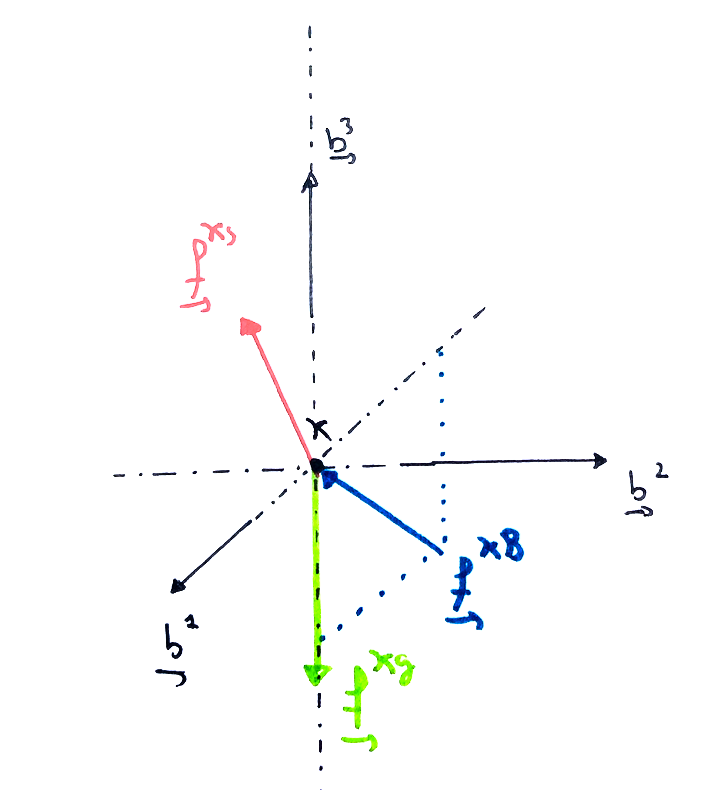
\includegraphics[width=\linewidth]{FBDk}
  \caption{FBD of $\kappa$.}
  \label{fig:FBDk}
\end{minipage}
\hspace{.05\linewidth}
\begin{minipage}{.42\linewidth}
  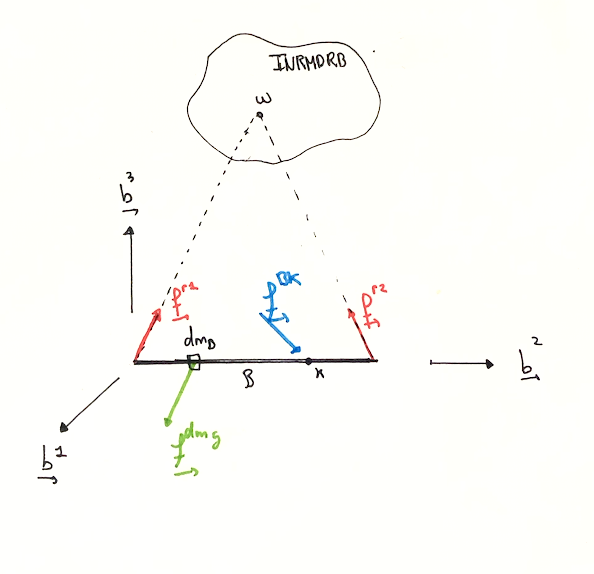
\includegraphics[width=\linewidth]{FBDB}
  \caption{FBD of $\mathcal{B}$.}
  \label{fig:FBDB}
\end{minipage}
\end{figure}

The norm of $\ura{r}^{\kappa w}$ is 
$$\vert\vert \ura{r}^{\kappa w}\vert\vert_2={\mbf{r}_b^{\kappa w}}^\trans\mbf{r}_b^{\kappa w}=y^2+d^2.$$
Therefore, the total force applied on $\kappa$ is given by:
\begin{align*}
\ura{f}^{\kappa}&=\ura{f}^{\kappa\mathcal{B}}+\ura{f}^{\kappa g}+\ura{f}^{\kappa s}
\\&=\vectrix{b}^\trans\left(\colvec{f_{b1}^{\kappa\mathcal{B}}}{0}{f_{b3}^{\kappa\mathcal{B}}}+\vectrix{b}^\trans\Cone{\theta}\colvec{0}{0}{-m_{\kappa}g}-k\frac{l_s-\bar{l}_s}{y^2+d^2}\colvec{0}{y}{-d}\right)
\\&=
\vectrix{b}^\trans\colvec{f_{b1}^{\kappa \mathcal{B}}}{-m_{\kappa}g\sin(\theta)-ky\frac{l_s-\bar{l}_s}{y^2+d^2}}{f_{b3}^{\kappa \mathcal{B}}-m_{\kappa}g\cos(\theta)+kd\frac{l_s-\bar{l}_s}{y^2+d^2}}.
\end{align*}
The total force acting on $\mathcal{B}$ is given by:
\begin{align*}
\ura{f}^{\mathcal{B}}&=\ura{f}^{r1}+\ura{f}^{r2}+\ura{f}^{\mathcal{B}\kappa}+\int_{\mathcal{B}}d\ura{f}^{dmg}
\\&=\vectrix{b}^\trans\left(
\colvec{f_{b1}^{r1}}{f_{b2}^{r1}}{f_{b3}^{r1}}+\colvec{f_{b1}^{r2}}{f_{b2}^{r2}}{f_{b3}^{r3}}-\colvec{f_{b1}^{\kappa\mathcal{B}}}{0}{f_{b3}^{\kappa\mathcal{B}}}+\Cone{\theta}\int_{\mathcal{B}}\colvec{0}{0}{-g}dm
\right)
\\ = & \vectrix{b}^\trans\colvec
{f_{b1}^{r1}+f_{b1}^{r2}-f_{b1}^{\kappa\mathcal{B}}}
{f_{b2}^{r1}+f_{b2}^{r2}-m_{\mathcal{B}}g\sin(\theta)}
{f_{b3}^{r1}+f_{b3}^{r2}-f_{b3}^{\kappa\mathcal{B}}-m_{\mathcal{B}}g\cos(\theta)}.
\end{align*}
Finally, the total moment applied on $\mathcal{B}$ relative to $w$ is given by:
\begin{align*}
\ura{m}^{\mathcal{B}w}&=\underbrace{\ura{r}^{r1w}\times\ura{f}^{r1}}_{=\, \ura{0}}+\underbrace{\ura{r}^{r2w}\times\ura{f}^{r2}}_{=\, \ura{0}}+\ura{r}^{\kappa w}\times \ura{f}^{\mathcal{B} \kappa}+\int_{\mathcal{B}}\ura{r}^{dmw}\times d\ura{f}^{dmg}
\\ & =\ura{r}^{\kappa w}\times \ura{f}^{\mathcal{B} \kappa}+\underbrace{\left(\int_{\mathcal{B}}\ura{r}^{dmw}dm\right)}_{=m_{\mathcal{B}}\ura{r}^{cw}}\times\ura{g}
\\ & =\vectrix{b}^\trans\left( \colvec{0}{y}{-d}^\times\colvec{-f_{b1}^{\kappa\mathcal{B}}}{0}{-f_{b3}^{\kappa\mathcal{B}}}+m_{\mathcal{B}}\colvec{0}{0}{-d}^\times\Cone{\theta}\colvec{0}{0}{-g}\right)
\\ & =
\vectrix{b}^\trans\colvec
{-yf_{b3}^{\kappa\mathcal{B}}-dgm_{\mathcal{B}}\sin(\theta)}
{df_{b1}^{\kappa\mathcal{B}}}
{yf_{b1}^{\kappa\mathcal{B}}}
\end{align*}

\paragraph{c)}

\begin{align*}
\ura{p}^{\kappa w/a}=m_{\kappa}{\ura{r}^{\kappa w/a}}^\fdot{a}=m_{\kappa}\vectrix{b}^\trans\colvec{0}{\dot{y}+d\dot{\theta}}{y\dot{\theta}}=\colvec{0}{m_{\kappa}(\dot{y}+d\dot{\theta})}{m_{\kappa}y\dot{\theta}}.\quad \Box
\end{align*}

\begin{align*}
\ura{h}^{\mathcal{B}w/a}
&=
\int_{\mathcal{B}}\ura{r}^{dmw}\times{\ura{r}^{dmw}}^\fdot{a}dm
\\ & = 
\vectrix{b}^\trans\left(\int_{\mathcal{B}}\colvec{\rho_{b1}}{\rho_{b2}}{\rho_{b3}-d}^\times\colvec{0}{(d-\rho_{b3})\dot{\theta}}{\rho_{b2}\dot{\theta}}dm\right)
\\ & =
\vectrix{b}^\trans\left(\int_{\mathcal{B}}\crossop{\rho_{b1}}{\rho_{b2}}{(\rho_{b3}-d)}\colvec{0}{(d-\rho_{b3})\dot{\theta}}{\rho_{b2}\dot{\theta}}dm\right)
\\ & =
\vectrix{b}^\trans\left(\dot{\theta}\int_{\mathcal{B}}\colvec
{(d-\rho_{b3})^2+\rho_{b2}^2}
{-\rho_{b1}\rho_{b2}}
{\rho_{b1}(d-\rho_{b3})}
dm\right)
\\ & =
\vectrix{b}^\trans\left(\dot{\theta}\int_{V_\mathcal{B}}\colvec
{(d-\rho_{b3})^2+\rho_{b2}^2}
{-\rho_{b1}\rho_{b2}}
{\rho_{b1}(d-\rho_{b3})}
\left(\frac{m_\mathcal{B}}{lth}\right)dV\right)
\\ & =
\vectrix{b}^\trans\left(\frac{m_\mathcal{B}\dot{\theta}}{lth}\colvec
{lt[\int_{-h/2}^{h/2}(d-\rho_{b3})^2d\rho_{b3}]+th[\int_{-l/2}^{l/2}\rho_{b2}^2d\rho_{b2}]}
{-lth^2[\underbrace{\int_{-t/2}^{t/2}\rho_{b1}d\rho_{b1}}_{0}][\underbrace{\int_{-l/2}^{l/2}\rho_{b2}d\rho_{b2}}_{0}]}
{l^2ht[\underbrace{\int_{-t/2}^{t/2}\rho_{b1}d\rho_{b1}}_{0}][\int_{-h/2}^{h/2}(d-\rho_{b3})d\rho_{b3}]}
\right)
\\ & =
\vectrix{b}^\trans\left(\frac{m_\mathcal{B}\dot{\theta}}{lth}\colvec
{-\frac{lt}{3}[(d-\rho_{b3})^3]_{-h/2}^{h/2}+\frac{th}{3}[\rho_{b2}^3]_{-l/2}^{l/2}}
{0}
{0}
\right)
\\ & =
\vectrix{b}^\trans\left(\frac{m_\mathcal{B}\dot{\theta}}{lth}\colvec
{-\frac{lt}{3}[-3d^2h-\frac{h^3}{4}]+\frac{th}{3}\frac{l^3}{4}}
{0}
{0}
\right)
\\ & =
\vectrix{b}^\trans\left(m_\mathcal{B}\dot{\theta}\colvec
{d^2+\frac{1}{12}(h^2+l^2)}
{0}
{0}
\right). \quad \Box
\end{align*}

\paragraph{d)}
First, from N2L,
\bdis
{\ura{p}^{\kappa w/a}}^\fdot{a}=\ura{f}^{\kappa}.
\edis
Using the Transport Theorem and developing:
\begin{align*}
{\ura{p}^{\kappa w/a}}^\fdot{a}
&={\ura{p}^{\kappa w/a}}^\fdot{b}+\ura{\omega}^{ba}\times{\ura{p}^{\kappa w/a}}
\\ & =
\vectrix{b}^\trans\left(\colvec
{0}
{m_{\kappa}(\ddot{y}+d\ddot{\theta})}
{m_{\kappa}(\dot{y}\dot{\theta}+y\ddot{\theta})}+\colvec{\dot{\theta}}{0}{0}^\times
\colvec
{0}
{m_{\kappa}(\dot{y}+d\dot{\theta})}
{m_{\kappa}y\dot{\theta}}
\right)
\\ & =
\vectrix{b}^\trans\colvec
{0}
{m_{\kappa}(\ddot{y}+d\ddot{\theta})-m_\kappa y\dot{\theta}^2}
{m_{\kappa}(\dot{y}\dot{\theta}+y\ddot{\theta})+\dot{\theta}m_{\kappa}(\dot{y}+d\dot{\theta})}
\\ & =
\vectrix{b}^\trans\colvec
{0}
{m_{\kappa}(\ddot{y}+d\ddot{\theta})-m_\kappa y\dot{\theta}^2}
{2m_{\kappa}\dot{y}\dot{\theta}+m_\kappa y\ddot{\theta}+m_\kappa d\dot{\theta}^2)}
\end{align*}
Therefore,
\beq
\colvec
{0}
{m_{\kappa}(\ddot{y}+d\ddot{\theta})-m_\kappa y\dot{\theta}^2}
{2m_{\kappa}\dot{y}\dot{\theta}+m_\kappa y\ddot{\theta}+m_\kappa d\dot{\theta}^2)}
=
\colvec{f_{b1}^{\kappa \mathcal{B}}}
{-m_{\kappa}g\sin(\theta)-ky\frac{l_s-\bar{l}_s}{y^2+d^2}}
{{f_{b3}^{\kappa \mathcal{B}}}-m_{\kappa}g\cos(\theta)+kd\frac{l_s-\bar{l}_s}{y^2+d^2}}.
\label{eq:DE1}
\eeq
We can see straight away that
$$f_{b1}^{\kappa \mathcal{B}}=0.$$
Secondly,
\begin{align*}
{\ura{h}^{\mathcal{B}w/a}}^\fdot{a}
&={\ura{h}^{\mathcal{B}w/a}}^\fdot{b}+\ura{\omega}^{ba}\times{\ura{h}^{\mathcal{B}w/a}}
\\ & =
\vectrix{b}^\trans\left(\colvec
{ m_\mathcal{B}\ddot{\theta}[d^2+\frac{1}{12}(h^2+l^2)]}
{0}
{0}
+
\colvec{\dot{\theta}}{0}{0}^\times
\colvec
{ m_\mathcal{B}\dot{\theta}[d^2+\frac{1}{12}(h^2+l^2)]}
{0}
{0}
\right)
\\ & =
\vectrix{b}^\trans\colvec
{ m_\mathcal{B}\ddot{\theta}[d^2+\frac{1}{12}(h^2+l^2)]}
{0}
{0}.
\end{align*}

From N2LR,
\bdis
{\ura{h}^{\mathcal{B}w/a}}^\fdot{a}=\ura{m}^{\mathcal{B}w}.
\edis
Therefore,
\bdis
\vectrix{b}^\trans\colvec
{ m_\mathcal{B}\ddot{\theta}[d^2+\frac{1}{12}(h^2+l^2)]}
{0}
{0}
=
\vectrix{b}^\trans\colvec
{-yf_{b3}^{\kappa\mathcal{B}}-dgm_{\mathcal{B}}\sin(\theta)}
{df_{b1}^{\kappa\mathcal{B}}}
{yf_{b1}^{\kappa\mathcal{B}}}
\edis
In particular,
\beq
f_{b3}^{\kappa\mathcal{B}}=-\frac{m_\mathcal{B}}{y}\left(\ddot{\theta}[d^2+\frac{1}{12}(h^2+l^2)]+dg\sin(\theta)\right)
\label{eq:fb3kB}
\eeq
Finally, substituting \eqref{eq:fb3kB} into \eqref{eq:DE1},
\begin{align}
m_{\kappa}(\ddot{y}+d\ddot{\theta})-m_\kappa y\dot{\theta}^2  &= -m_{\kappa}g\sin(\theta)-ky\frac{l_s-\bar{l}_s}{y^2+d^2} \label{eq:DE2} \\
2m_{\kappa}\dot{y}\dot{\theta}+m_\kappa y\ddot{\theta}+m_\kappa d\dot{\theta}^2  &= -\frac{m_\mathcal{B}}{y}\left(\ddot{\theta}[d^2+\frac{1}{12}(h^2+l^2)]+dg\sin(\theta)\right) \nonumber \\ & -m_{\kappa}g\cos(\theta)+kd\frac{l_s-\bar{l}_s}{y^2+d^2} \label{eq:DE3}
\end{align}

\paragraph{e)}
The total moment applied on $\mathcal{S}$ relative to $w$ is given by:
\begin{align*}
\ura{m}^{\mathcal{S}w}=&m_\mathcal{B}\ura{r}^{cw}\times\ura{g}+m_\kappa \ura{r}^{\kappa w}\times \ura{g}
\\ & = \vectrix{b}^\trans\left(
m_\mathcal{B}\colvec{0}{0}{-d}^\times\colvec{0}{-\sin(\theta)g}{-\cos(\theta)g}
+m_\kappa\colvec{0}{y}{-d}^\times\colvec{0}{-\sin(\theta)g}{-\cos(\theta)g}
\right)
\\ & =
\vectrix{b}^\trans\colvec
{-m_\mathcal{B}dg\sin(\theta)+m_\kappa[-yg\cos(\theta)-dg\sin(\theta)]}
{0}
{0}. \quad \Box
\end{align*}
Secondly,
\begin{align*}
\ura{h}^{\mathcal{S}w/a}&=\ura{h}^{\mathcal{B}w/a}+\ura{r}^{\kappa w}\times \ura{p}^{\kappa w / a}
\\ & = \vectrix{b}^\trans\left(
\colvec
{ m_\mathcal{B}\dot{\theta}[d^2+\frac{1}{12}(h^2+l^2)]}
{0}
{0}
+ \colvec{0}{y}{-d}^\times
\colvec{0}{m_{\kappa}(\dot{y}+d\dot{\theta})}{m_{\kappa}y\dot{\theta}}
\right)
\\ & =
\vectrix{b}^\trans
\colvec
{ m_\mathcal{B}\dot{\theta}[d^2+\frac{1}{12}(h^2+l^2)]+m_\kappa[y^2\dot{\theta}+d(\dot{y}+d\dot{\theta})]}
{0}
{0}.
\end{align*}
Therefore,
\begin{align*}
{\ura{h}^{\mathcal{S}w/a}}^\fdot{a}&=
{\ura{h}^{\mathcal{S}w/a}}^\fdot{b}+\underbrace{\ura{\omega}^{ba}\times\ura{h}^{\mathcal{S}w/a}}_{=\,\ura{0}}
\\ & =
\vectrix{b}^\trans
\colvec
{ m_\mathcal{B}\ddot{\theta}[d^2+\frac{1}{12}(h^2+l^2)]+m_\kappa[2y\dot{y}\dot{\theta}+y^2\ddot{\theta}+d(\ddot{y}+d\ddot{\theta})]}
{0}
{0}.
\end{align*}
And finally, applying N2LR, i.e. ${\ura{h}^{\mathcal{S}w/a}}^\fdot{a}=\ura{m}^{\mathcal{S}w}$:
\begin{align}
m_\mathcal{B}\ddot{\theta}[d^2+\frac{1}{12}(h^2+l^2)]&+m_\kappa[2y\dot{y}\dot{\theta}+y^2\ddot{\theta}+d(\ddot{y}+d\ddot{\theta})]
 \nonumber \\& =
-m_\mathcal{B}dg\sin(\theta)+m_\kappa[-yg\cos(\theta)-dg\sin(\theta)]
\label{eq:DE4}
\end{align}
We can easily check that \eqref{eq:DE4} is nothing else than $d\cdot$\eqref{eq:DE2} + $y\cdot$\eqref{eq:DE3}, and thus the two sets of DEs describe the same motion.

% Question 3-------------------------------------------------------------------------------------------------------------------------------------------------------
\section*{3}
\paragraph{a)}
\begin{align*}
\ura{\omega}^{sa}&=\ura{\omega}^{sb}+\ura{\omega}^{bq}+\ura{\omega}^{qa}
\\ & =
\vectrix{s}^\trans\mbs{\omega}_s^{sb} + \vectrix{b}^\trans\mbs{\omega}_b^{bq} + \vectrix{q}^\trans\mbs{\omega}_q^{qa}
\\ & =
\vectrix{s}^\trans\mbs{\omega}_s^{sb} + \vectrix{s}^\trans\mbf{C}_{sb}\mbs{\omega}_b^{bq} + \vectrix{s}^\trans\mbf{C}_{sq}\mbs{\omega}_q^{qa}
\\ & =
\vectrix{s}^\trans\mbs{\omega}_s^{sb} + \vectrix{s}^\trans\mbf{C}_3(\gamma)\mbs{\omega}_b^{bq} + \vectrix{s}^\trans\mbf{C}_3(\gamma)\mbf{C}_2(\phi)\mbs{\omega}_q^{qa}
\\ & =
\vectrix{s}^\trans\left(\mbf{1}_3\dot{\gamma} + \mbf{C}_3(\gamma)\mbf{1}_2\dot{\phi} + \mbf{C}_3(\gamma)\mbf{C}_2(\phi)\mbf{1}_3\dot{\theta}\right)
\\ & =
\vectrix{s}^\trans\underbrace{\rowvec{\mbf{C}_3(\gamma)\mbf{C}_2(\phi)\mbf{1}_3}
{\mbf{C}_3(\gamma)\mbf{1}_2}
{\mbf{1}_3}
\colvec{\dot{\theta}}{\dot{\phi}}{\dot{\gamma}}}_{\mbs{\omega}_s^{sa}}. \quad \Box
\end{align*}

\paragraph{b)}
\begin{align*}
{\ura{r}^{\dif m w}}^\fdot{a} &=
\left(\ura{r}^{\dif m c}+\ura{r}^{c w}\right)^\fdot{a}
\\ & =
\left(\ura{r}^{\dif m c}+\ura{r}^{c w}\right)^\fdot{s}+\ura{\omega}^{sa} \times \left(\ura{r}^{\dif m c}+\ura{r}^{c w}\right)
\\ & =
\vectrix{s}^\trans\left(\underbrace{\dot{\mbf{r}}_s^{\dif m c}}_{=\mbf{0}}+\underbrace{\dot{\mbf{r}}_s^{cw}}_{=\mbf{0}}\right)+\ura{\omega}^{sa} \times \left(\ura{r}^{\dif m c}+\ura{r}^{c w}\right)
\\ & = 
\ura{\omega}^{sa} \times \left(\ura{r}^{\dif m c}+\ura{r}^{c w}\right). \quad \Box
\end{align*}
Where we've used the facts that the material element $\dif m$ is fixed in the body frame $\mathcal{F}_s$ and that $\dot{\mbf{r}}_s^{cw}=\dot{l}\mbf{1}_3=\mbf{0}$.

\paragraph{c)}
\begin{align*}
\ura{h}^{\mathcal{B}w/a}&= 
\int_{\mathcal{B}}\ura{r}^{\dif m w}\times{\ura{r}^{\dif m w}}^\fdot{a} \dif m
\\ & =
\int_{\mathcal{B}}\ura{r}^{\dif m w}\times\left[\ura{\omega}^{sa} \times \left(\ura{r}^{\dif m c}+\ura{r}^{c w}\right)\right] \dif m
\\ & =
\int_{\mathcal{B}}\left(\ura{r}^{\dif m c}+\ura{r}^{c w}\right)\times\left[\ura{\omega}^{sa} \times \ura{r}^{\dif m c}+\ura{\omega}^{sa}\times\ura{r}^{c w}\right] \dif m
\\ & =
\int_{\mathcal{B}}\left(\ura{r}^{\dif m c}+\ura{r}^{c w}\right)\times\left[- \ura{r}^{\dif m c}\times\ura{\omega}^{sa}-\ura{r}^{c w}\times\ura{\omega}^{sa}\right] \dif m
\\ & =
\int_{\mathcal{B}}-\ura{r}^{\dif m c}\times(\ura{r}^{\dif m c}\times\ura{\omega}^{sa})-\ura{r}^{\dif m c}\times(\ura{r}^{c w}\times\ura{\omega}^{sa})
\\ & \qquad -\ura{r}^{c w}\times(\ura{r}^{\dif m c}\times\ura{\omega}^{sa})-\ura{r}^{c w}\times(\ura{r}^{c w}\times\ura{\omega}^{sa}) \dif m
\\ & =
\int_{\mathcal{B}}-\ura{r}^{\dif m c}\times(\ura{r}^{\dif m c}\times\ura{\omega}^{sa})
+(\ura{r}^{c w}\times\ura{\omega}^{sa})\times\ura{r}^{\dif m c}
\\ & \qquad +\ura{r}^{c w}\times(\ura{\omega}^{sa}\times\ura{r}^{\dif m c})
-\ura{r}^{c w}\times(\ura{r}^{c w}\times\ura{\omega}^{sa}) \dif m
\\ & =
\vectrix{s}^\trans\left\{ \int_{\mathcal{B}}
-{\mbf{r}_s^{\dif m c}}^\times{\mbf{r}_s^{\dif m c}}^\times\mbs{\omega}_s^{sa}
+({\mbf{r}_s^{cw}}^\times\mbs{\omega}_s^{sa})^\times\mbf{r}_s^{\dif m c}
+{\mbf{r}_s^{cw}}^\times{\mbs{\omega}_s^{sa}}^\times\mbf{r}_s^{\dif m c}
-{\mbf{r}_s^{cw}}^\times{\mbf{r}_s^{cw}}^\times\mbs{\omega}_s^{sa}
\dif m \right\}
\\ & =
\vectrix{s}^\trans\left\{ 
\underbrace{\left[\int_{\mathcal{B}}-{\mbf{r}_s^{\dif m c}}^\times{\mbf{r}_s^{\dif m c}}^\times \dif m\right]}_{\mbf{J}_s^{\mathcal{B}c}}\mbs{\omega}_s^{sa}
+\left[({\mbf{r}_s^{cw}}^\times\mbs{\omega}_s^{sa})^\times+{\mbf{r}_s^{cw}}^\times{\mbs{\omega}_s^{sa}}^\times\right]\underbrace{\int_{\mathcal{B}}\mbf{r}_s^{\dif m c} \dif m}_{\mbf{0}} \right.
\\ & \left . \qquad
+\underbrace{\overbrace{\int_{\mathcal{B}}\dif m}^{m_\mathcal{B}} \left[-{\mbf{r}_s^{cw}}^\times{\mbf{r}_s^{cw}}^\times\right]}_{\mbf{J}_s^{m_\mathcal{B}w}}\mbs{\omega}_s^{sa}
 \right\}
 \\ & =
 \vectrix{s}^\trans\left\{(\mbf{J}_s^{\mathcal{B}c}+\mbf{J}_s^{m_\mathcal{B}w})\mbs{\omega}_s^{sa}
 \right\}
 \\ & =
 (\ura{J}^{\mathcal{B}c}+\ura{J}^{m_\mathcal{B}w})\cdot\ura{\omega}^{sa}
 \\ & = \ura{J}^{\mathcal{B}w}\cdot\ura{\omega}^{sa}. \quad \Box
\end{align*}

\paragraph{e)}
From ERL,
\beq
{\ura{h}^{\mathcal{B}w/a}}^\fdot{a}=\ura{m}^{\mathcal{B}w}.
\label{eq:ERL}
\eeq
Developing on both sides:
\begin{align*}
{\ura{h}^{\mathcal{B}w/a}}^\fdot{a}&={\ura{h}^{\mathcal{B}w/a}}^\fdot{s}+\ura{\omega}^{sa}\times{\ura{h}^{\mathcal{B}w/a}}
\\ & =
\left\{\vectrix{s}^\trans(\mbf{J}_s^{\mathcal{B}c}+\mbf{J}_s^{m_\mathcal{B}w})\mbs{\omega}_s^{sa}\right\}^\fdot{s}+\vectrix{b}^\trans{\mbs{\omega}_s^{sa}}^\times(\mbf{J}_s^{\mathcal{B}c}+\mbf{J}_s^{m_\mathcal{B}w})\mbs{\omega}_s^{sa}
\\ & =
\vectrix{s}^\trans\left\{
\underbrace{(\dot{\mbf{J}}_s^{\mathcal{B}c}+\dot{\mbf{J}}_s^{m_\mathcal{B}w})}_{=\mbf{0} \mbox{\footnotesize{ (Body frame)}}}\mbs{\omega}_s^{sa}+(\mbf{J}_s^{\mathcal{B}c}+\mbf{J}_s^{m_\mathcal{B}w})\dot{\mbs{\omega}}_s^{sa}+{\mbs{\omega}_s^{sa}}^\times(\mbf{J}_s^{\mathcal{B}c}+\mbf{J}_s^{m_\mathcal{B}w})\mbs{\omega}_s^{sa}
\right\}
\\ & =
\vectrix{s}^\trans\left\{
(\mbf{J}_s^{\mathcal{B}c}+\mbf{J}_s^{m_\mathcal{B}w})\dot{\mbs{\omega}}_s^{sa}+{\mbs{\omega}_s^{sa}}^\times(\mbf{J}_s^{\mathcal{B}c}+\mbf{J}_s^{m_\mathcal{B}w})\mbs{\omega}_s^{sa}
\right\} \overset{\eqref{eq:ERL}}{=}
\vectrix{s}^\trans\mbf{m}_s^{\mathcal{B}w}. \quad \Box
\end{align*}

\paragraph{f)}
We have previously shown the following:
\begin{align*}
\mbs{\omega}_s^{sa}&=\mbf{S}_s^{sa}\dot{\mbs{\theta}}^{sa}, \\
(\mbf{J}_s^{\mathcal{B}c}+\mbf{J}_s^{m_\mathcal{B}w})\dot{\mbs{\omega}}_s^{sa}+{\mbs{\omega}_s^{sa}}^\times(\mbf{J}_s^{\mathcal{B}c}+\mbf{J}_s^{m_\mathcal{B}w})\mbs{\omega}_s^{sa}&=
\mbf{m}_s^{\mathcal{B}w}.
\end{align*}
Rearranging these equations:
\begin{align*}
\dot{\mbs{\theta}}^{sa} &=(\mbf{S}_s^{sa})^{-1}\mbs{\omega}_s^{sa},\\
\dot{\mbs{\omega}}_s^{sa}&=
(\mbf{J}_s^{\mathcal{B}c}+\mbf{J}_s^{m_\mathcal{B}w})^{-1}\left(\mbf{m}_s^{\mathcal{B}w}-{\mbs{\omega}_s^{sa}}^\times(\mbf{J}_s^{\mathcal{B}c}+\mbf{J}_s^{m_\mathcal{B}w})\mbs{\omega}_s^{sa}\right).
\end{align*}
Using the following notation,
\bdis
\mbf{x}=\colvec{\mbs{\theta}^{sa}}{\mbs{\omega}_s^{sa}}{}, \qquad \dot{\mbf{x}}=\colvec{\dot{\mbs{\theta}}^{sa}}{\dot{\mbs{\omega}}_s^{sa}}{},
\edis
we can write a first-order state-space system of the form
\bdis
\dot{\mbf{x}}=\mbf{f}(\mbf{x}).
\edis
Using \textsc{Matlab}{}, we obtain the following plots (the code is given at the end of the assignment):
\newpage

\begin{figure}[h!]
    \centering
        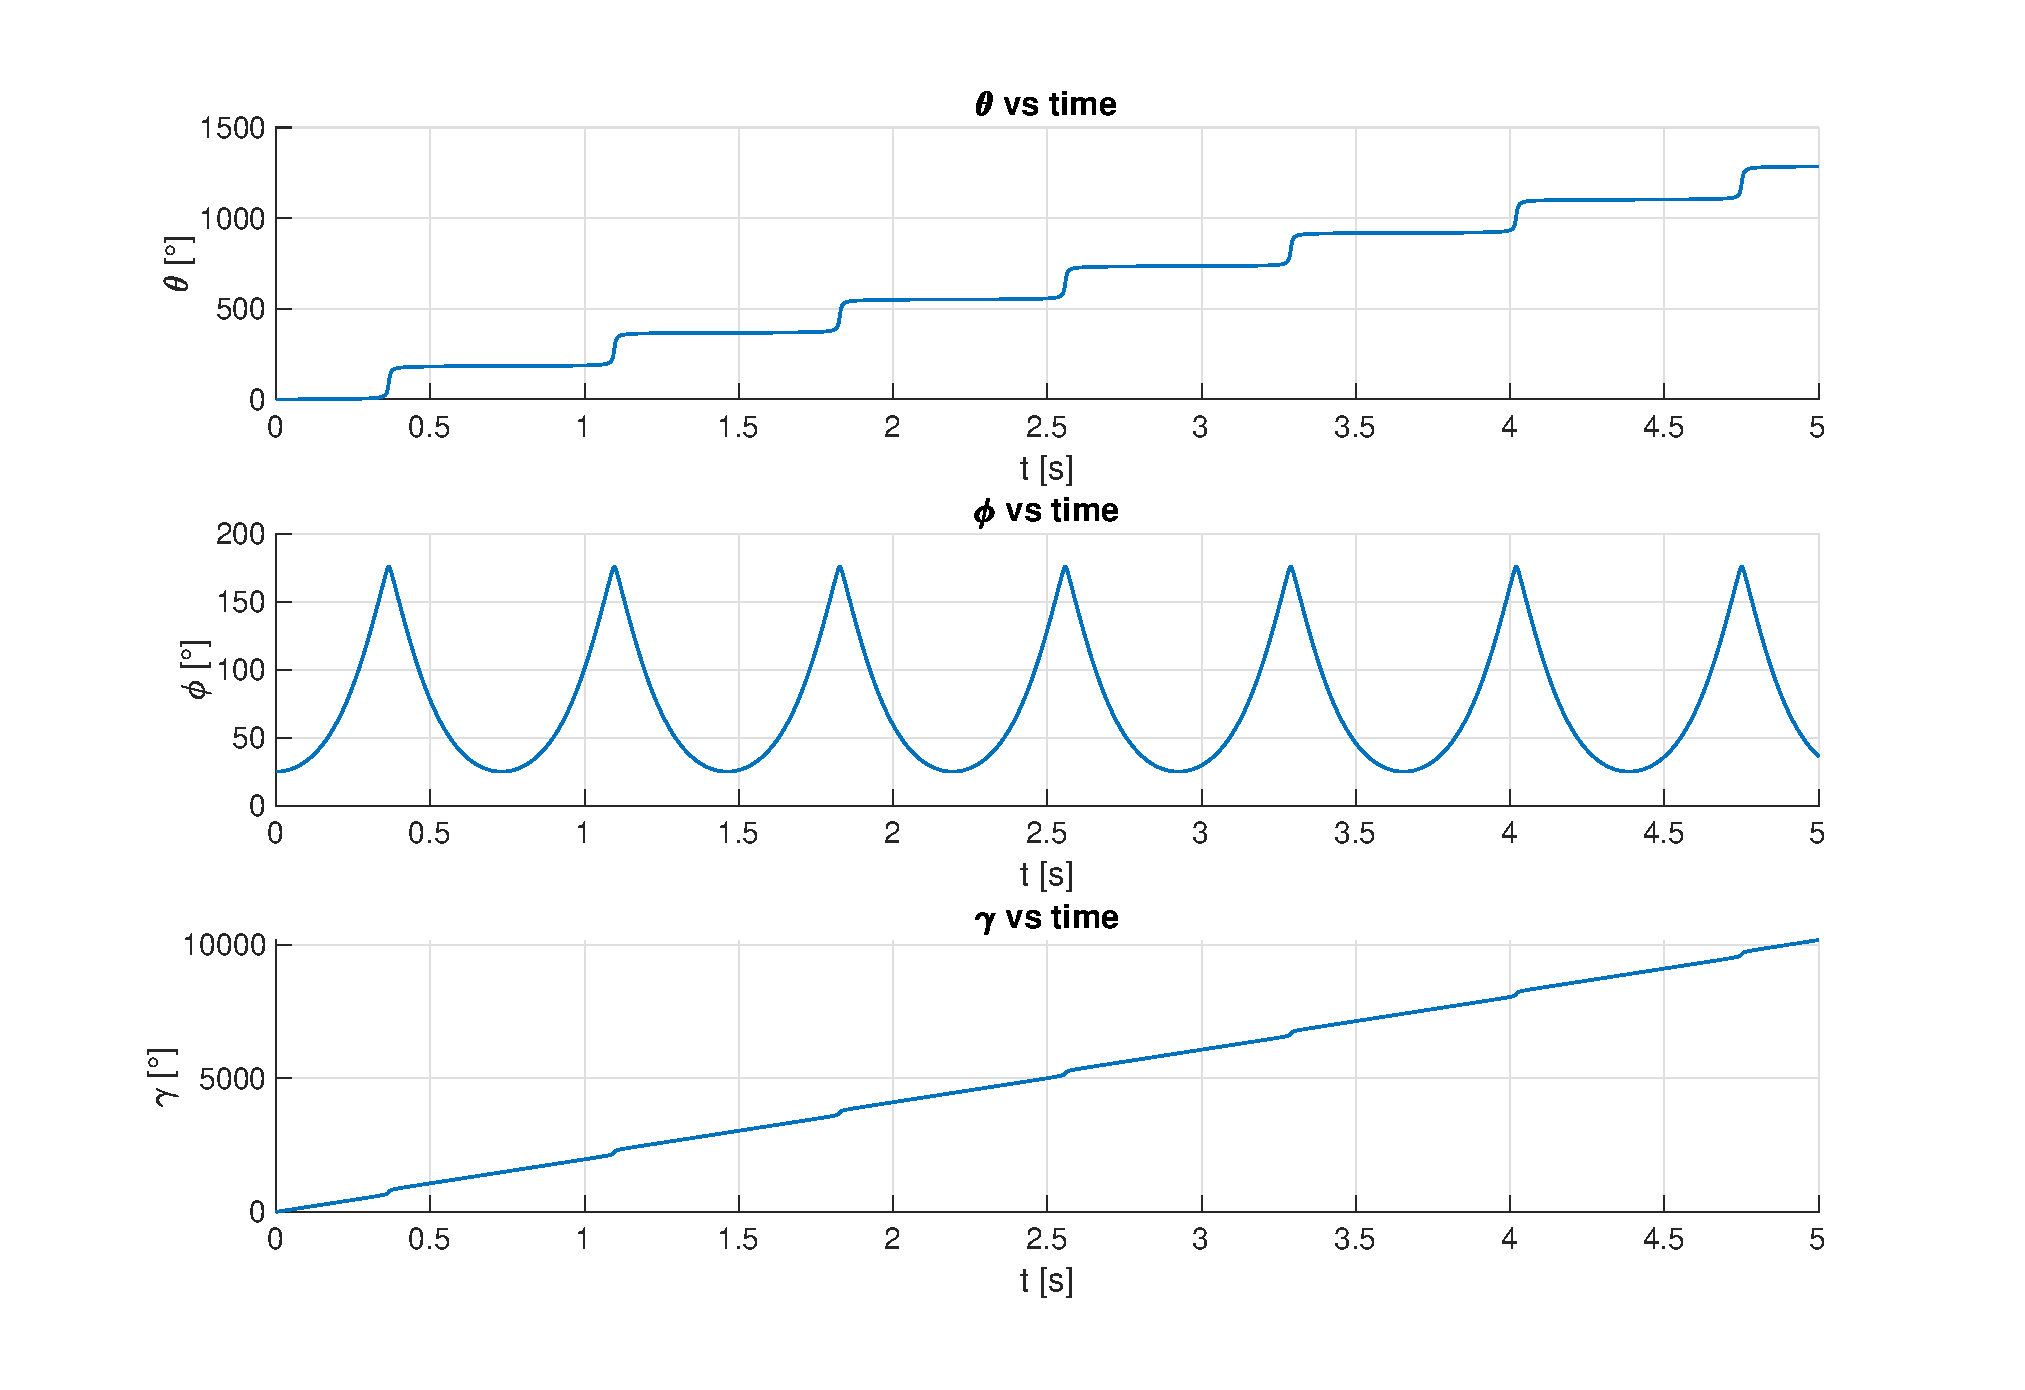
\includegraphics[width=.9\textwidth]{Ang}
    \caption{$\theta$, $\phi$ and $\gamma$ vs. time.}
    \label{fig:Ang}
%\end{figure}
%\begin{figure}[h]
    \centering
        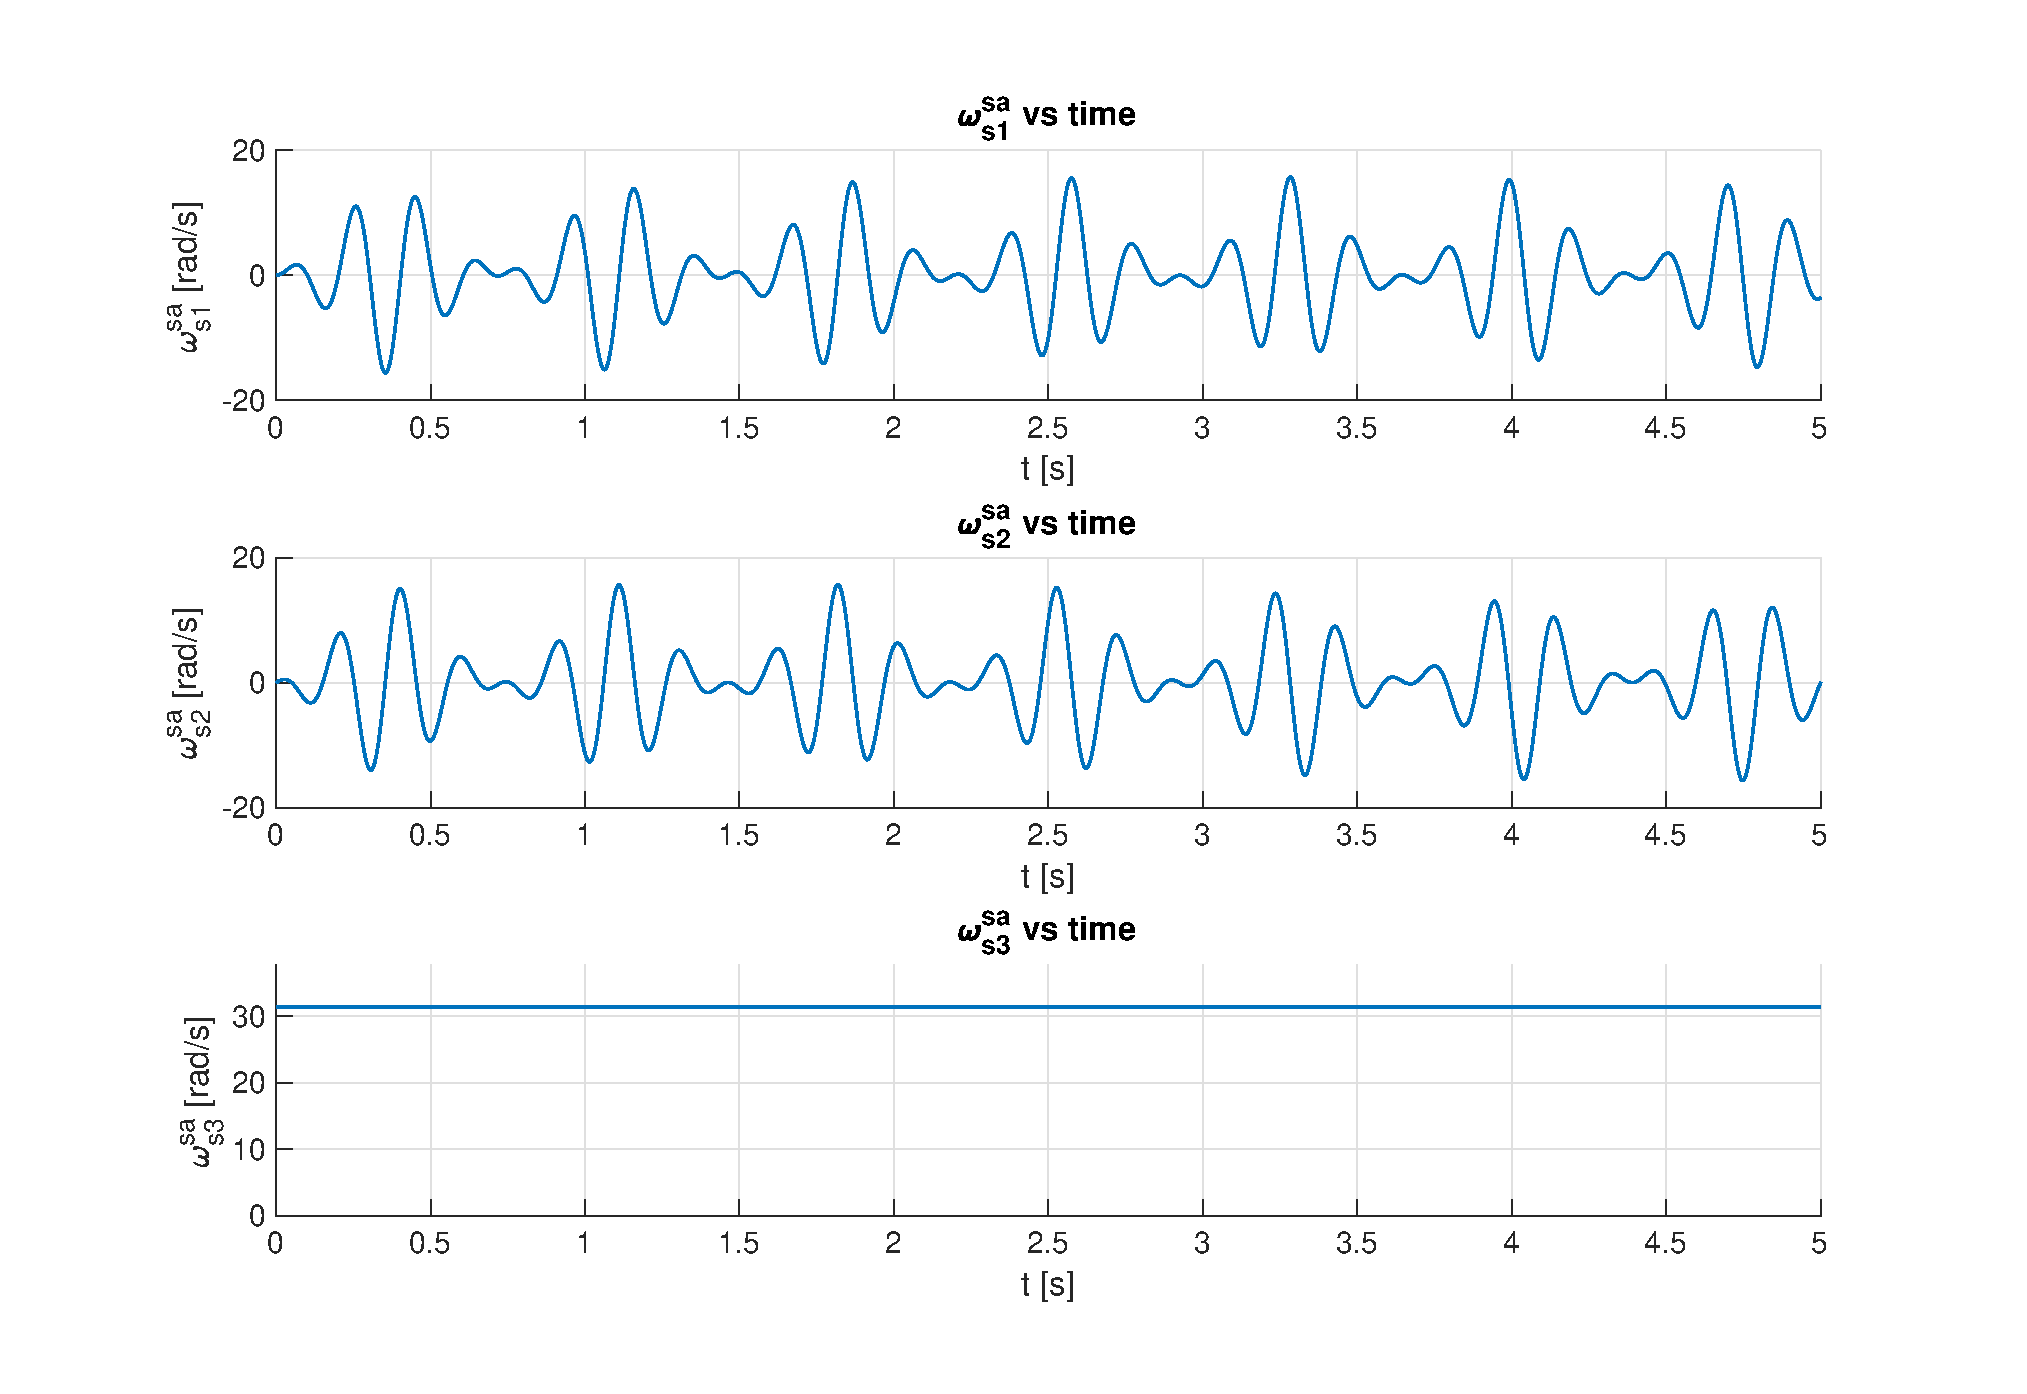
\includegraphics[width=.9\textwidth]{AngVel}
    \caption{$\omega_{s1}^{sa}$, $\omega_{s2}^{sa}$ and $\omega_{s3}^{sa}$ vs. time.}
    \label{fig:AngVel}
\end{figure}


\newpage 
\paragraph{g)}
First,
\begin{align*}
T_{\mathcal{B}w/a}&=\onehalf{\mbs{\omega}_s^{sa}}^\trans\mbf{J}_s^{\mathcal{B} w}\mbs{\omega}_s^{sa},
\\
U_{\mathcal{B}w}&=-\int_{\mathcal{B}}\ura{g}\cdot\ura{r}^{\dif m w}\dif m
\\ & = 
-\ura{g} \cdot\underbrace{\left(\int_{\mathcal{B}}\ura{r}^{\dif m w}\dif m\right)}_{\ura{r}^{cw}m_\mathcal{B}}
\\ & =
\left(\mbf{C}_3(\gamma)\mbf{C}_2(\phi)\mbf{C}_3(\theta)\mbf{1}_3g\right)^\trans\vectrix{s}\cdot\vectrix{s}^\trans\mbf{r}_s^{cw}m_\mathcal{B}
\\ & =
m_\mathcal{B}gl\left(\mbf{C}_3(\gamma)\mbf{C}_2(\phi)\mbf{C}_3(\theta)\mbf{1}_3\right)^\trans\mbf{1}_3.
\end{align*}
We can now use \textsc{Matlab}{} to obtain the plot shown in Figure \ref{fig:Energy}. As expected, $E_{\mathcal{B}w/a}$ is constant with time, which is a good indicator of an accurate simulation.
\begin{figure}[h!]
    \centering
        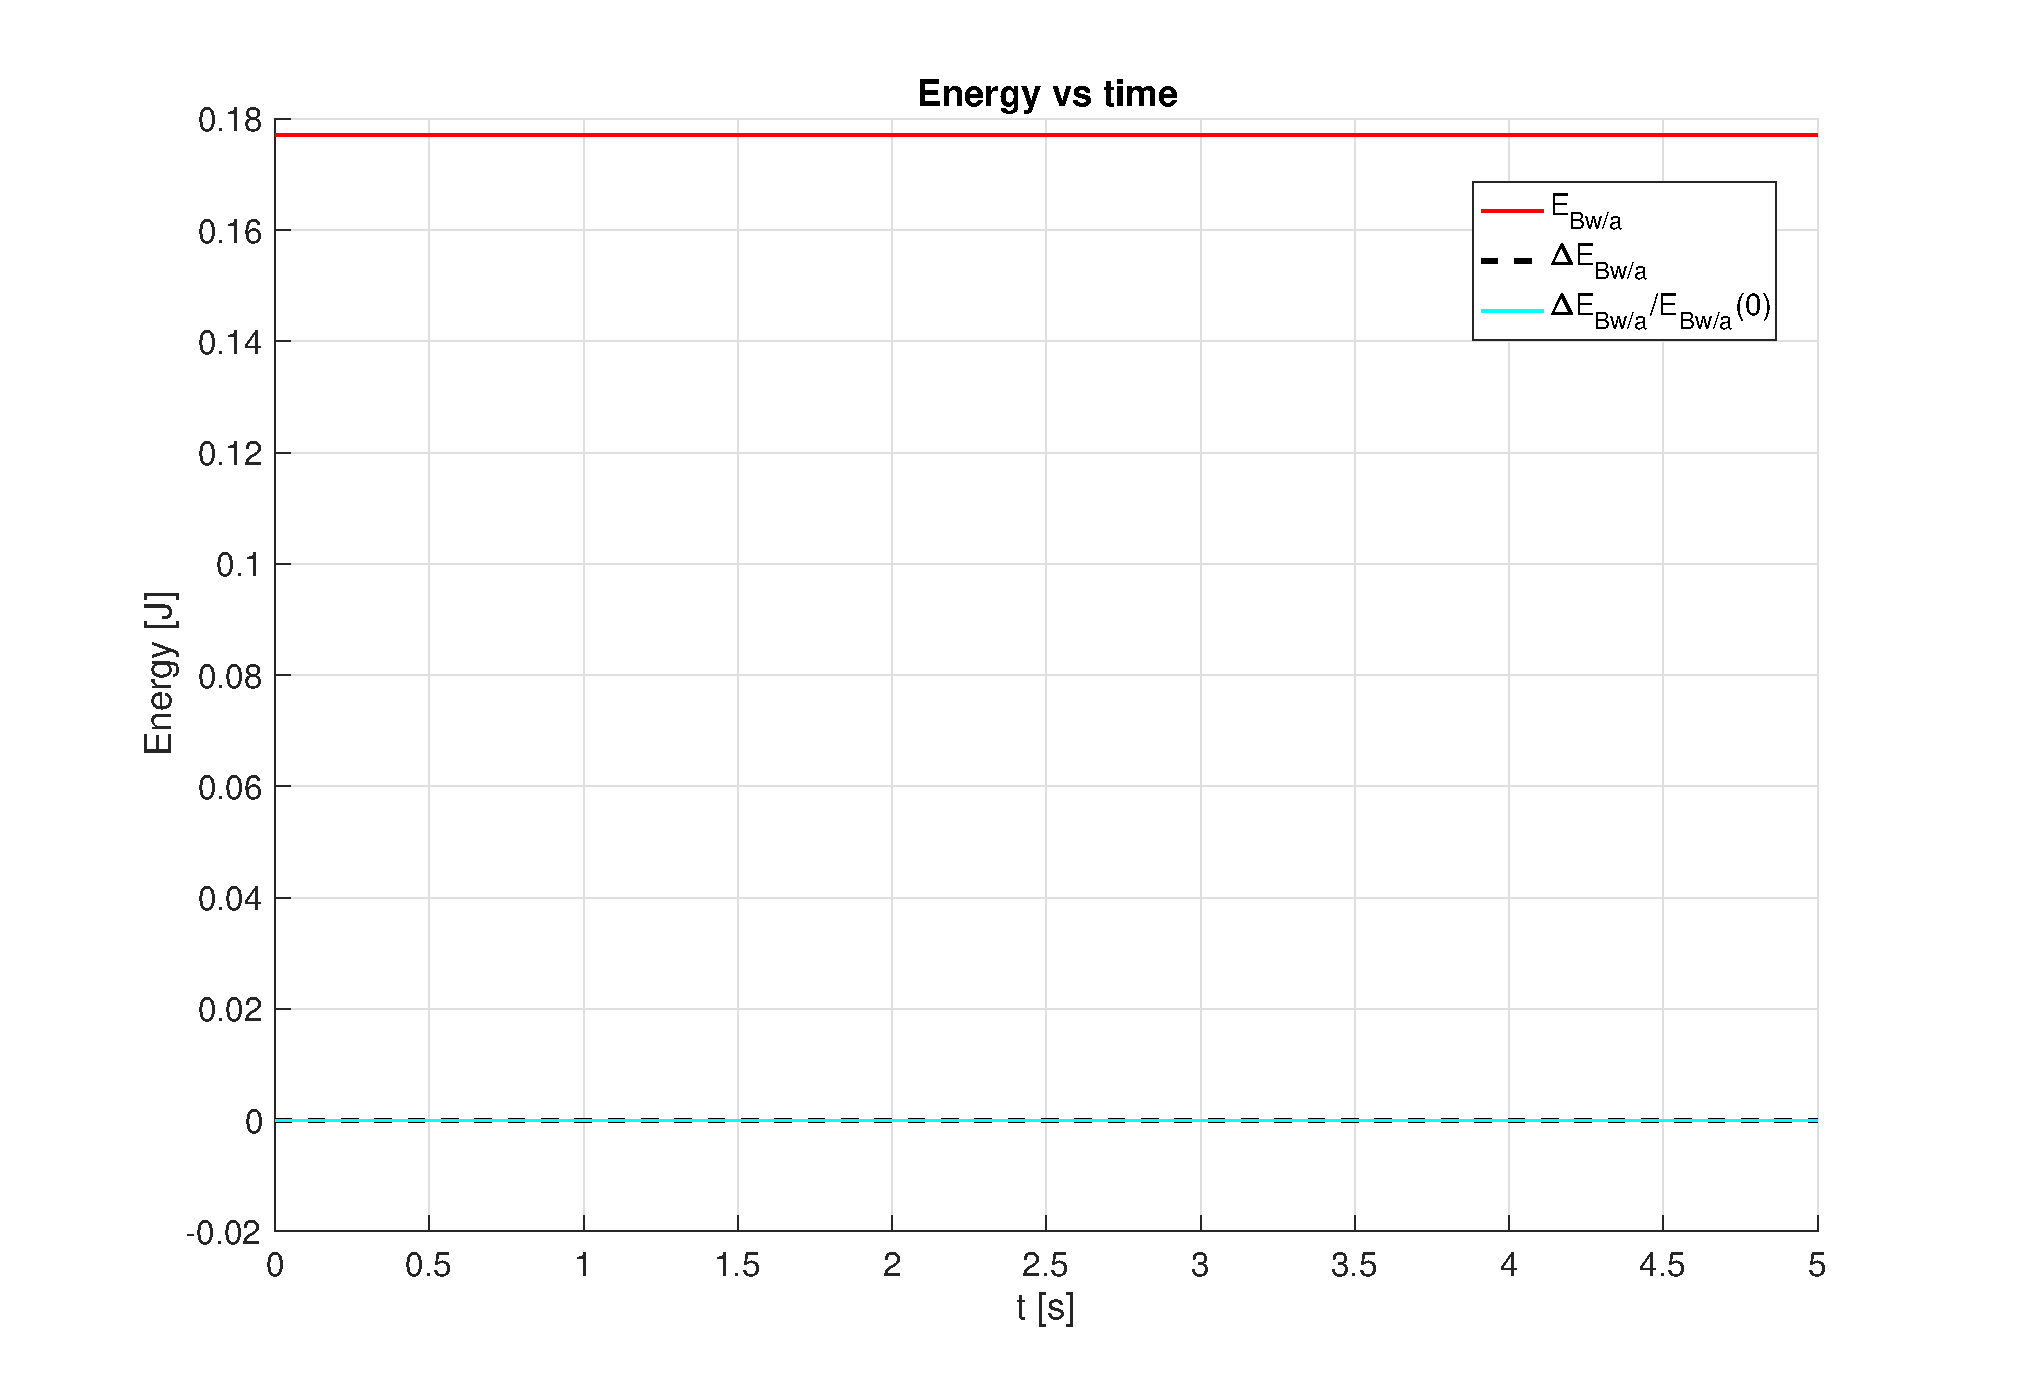
\includegraphics[width=1\textwidth]{Energy}
    \caption{Energy vs. time.}
    \label{fig:Energy}
\end{figure}

\end{document}


